% Канонический TikZ-рисунок варианта 28. Править только здесь.
\long\def\figStereoV28{%
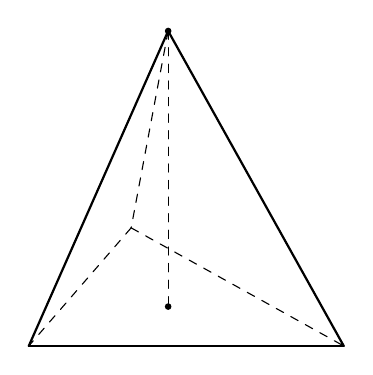
\begin{tikzpicture}[
  scale=1,
  line cap=round,
  line join=round
]
  % Основание
  \coordinate (A) at (0,0);
  \coordinate (B) at (4,0);
  \coordinate (C) at (1.3,1.5);

  % Центр основания
  \coordinate (O) at (1.77,0.5);

  % Вершина
  \coordinate (S) at (1.77,4);

  % Основание
  \draw[thick] (A)--(B);
  \draw[dashed] (C)--(B);
  \draw[dashed] (C)--(A);

  % Боковые рёбра
  \draw[thick] (S)--(A);
  \draw[thick] (S)--(B);
  \draw[dashed] (S)--(C);

  % Высота
  \draw[dashed] (S)--(O);

  \fill (S) circle (1.2pt);
  \fill (O) circle (1.2pt);
\end{tikzpicture}
}
